\documentclass[a4paper,12pt]{article}

\usepackage{graphicx}
\usepackage{ucs}
\usepackage[utf8x]{inputenc}
\PrerenderUnicode{åäöÅÄÖ}

\title{Costanza Userguide}
\author{M. Green, P. Krupinski, P. Melke, P. Sahlin, H. Jonsson}

\begin{document}

\maketitle

%\abstract 

\section{Introduction}

This document describes how to use COnfocal STack ANalyZer Application
(Costanza), an ImageJ\cite{Abramoff2004} plugin for analyzing confocal
stacks. The main purpose of Costanza is to segment nuclei marked cells
in three dimensions, making available quantitative measures such as
positions, sizes, and average intensities of GFP markers for the
segmented compartments. The main algorithm is independent of intensity
thresholds, allowing for segmentation of data of varying intensity.

Costanza assumes a greyscale stack of images as input, and work with
real length units and x, y, and z scales should be provided either via
ImageJ, or set by the user.

\section{Installation instructions}

In order to use Costanza you must have ImageJ
(http://rsb.info.nih.gov/ij) installed on your system. Download the
file Costanza.zip from
http://www.thep.lu.se/\{}~henrik/Costanza/. Unzip the Costanza archive
in the plugins directory of your ImageJ installation. Next time you
start ImageJ the plugin will show up as Costanza in the Plugins drop
down menu.

\section{Algorithms}

The algorithms privided in Costanza can be divided into the main
segmenter algorithm, preprocessing, and postprocessing.

\subsection{Steepest gradient descent for segmentation}

This is the main algorithm for Costanza. It starts at each voxel in the stacks
and tries to find local intensity maxima by ``walking'' uphill in intensity
among its neighbors. All paths leading to the same maxima are saved to the
basin of attractor of this maxima, and represents a compartment. If a neighbor
has an intensity value higher then the current voxel, a step is performed to
the neighbor with highest

\begin{equation}
\frac{\Delta I}{\Delta \mathbf{x}} =
\frac{I_{neigh}-I_{current}}{\mathbf{x}_{neigh}-\mathbf{x}_{current}}
\end{equation}

where $\mathbf{x}_{current}(\mathbf{x}_{current})$ is the current (neighbor)
position, and $I$ are the respective intensities.

The neighborhood is defined by the closest voxels, i.e
$(x\pm1,y,z)$, $(x,y\pm1,z)$, and $(x,y,z\pm1)$.


\subsection{Preprocessing}

\subsubsection{Intensity inversion}

Costanza assumes bright objects in a dark background. If the objects
are dark in a bright surrounding, the stack should be inverted. This
algorithm replaces each voxel intensity $I$ with its inverted value
$I_{max}-I$, where $I_{max}$ is the maximal value allowed in the
greyscale images. This algorithm does not require any user provided
parameter values.

\subsubsection{Background extraction by thresholding}

It may be benficial to remove voxels from treatment by the
segmentation algorithm. Both to remove uninteresting regions of the
stack, and for speeding up the algorithms. The background can be
extracted via a threshold filter, that assigns all voxels with
intensity $I$ less than a threshold value $I_{threshold}$ to belong to
the background, and will not be treated in the algorithms. The user
has to provide a value for the parameter $I_{threshold}$.

\subsubsection{Mean filter for smoothing}

Important for the segmentation to work is that the intensity noise is
low and the stack provided is smooth. This can be done by different
filters in ImageJ, but Costanza also provides a 3D filter for
smoothing. It uses a spherical XXX and replaces each voxel intensity
$I$ by an average calculated from all voxels with a center positioned
within a radius $R_{max}$ measured in real length. Since it can be
beneficial to run the filter multiple times with smaller $R_{max}$,
the user shopuld provide the two parameters, $R_{max}$ and the number
of times to run the filtering.

\subsection{Postprocessing}

After gradient descent is applied for segmentation, two post-processing steps
are available.

\subsubsection{Peak removal}

Since the gradient descent algorithm is insensitive to absolute intensity
values, it may happen that it finds compartments in the noisy
background. There is a post-processor for removing these false positives by
using thresholds in minimal size and minimal intensity for the extracted
compartments. The user should provide a minimal size $S_{min}$ given in volume
units, and minimal intensity $I_{min}$.

\subsubsection{Peak merging}

Bright objects with dark regions within them might be interpreted as several
compartments by the gradient descent algorithm. The user has the possibility
to merge such compartments, by setting a minimal distance
$R_{min}$. Compartments with centers at a distance below $R_{min}$ will be
merged into a single compartment. This algorithm is run recursively.


\section{User interface}

\subsection{Main}

The main menu is used for running the Costanza application by chosing ``Start
analyze''. The current active stack and selected processors and parameter
values will be used. The main menu also includes a ``close'' function that
will exit the Costanza plugin.

\subsection{Options}

Options are used to set all features of Costanza. Three different views can be
selected (Fig.~\ref{fig:gui}). 

\begin{figure}[h!]
\begin{center}
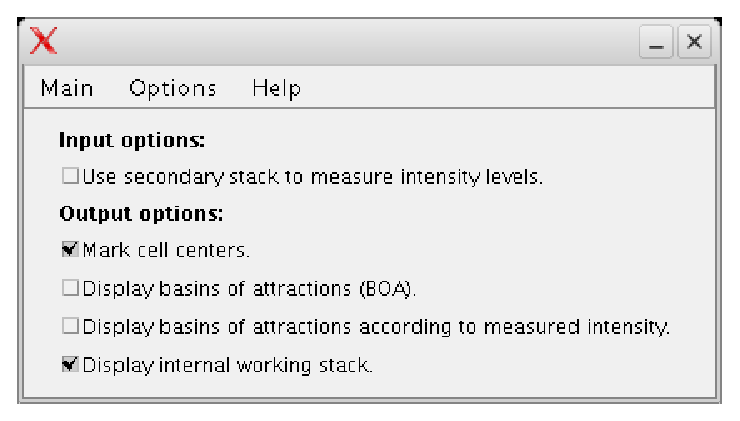
\includegraphics[width=0.5\columnwidth]{figures/GUI_input_output.eps}\\
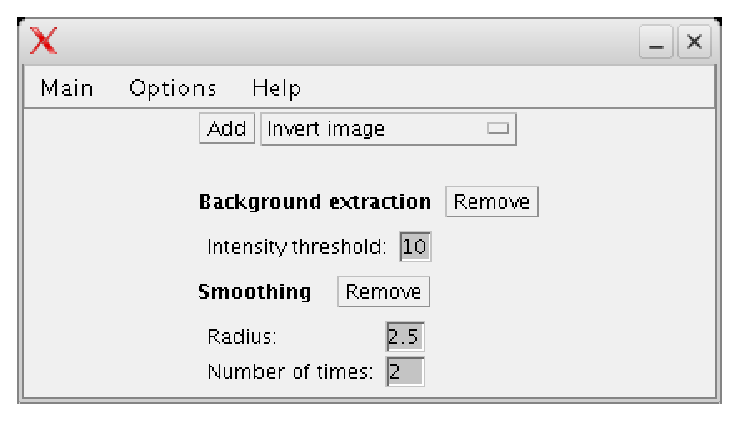
\includegraphics[width=0.5\columnwidth]{figures/GUI_pre.eps}\\
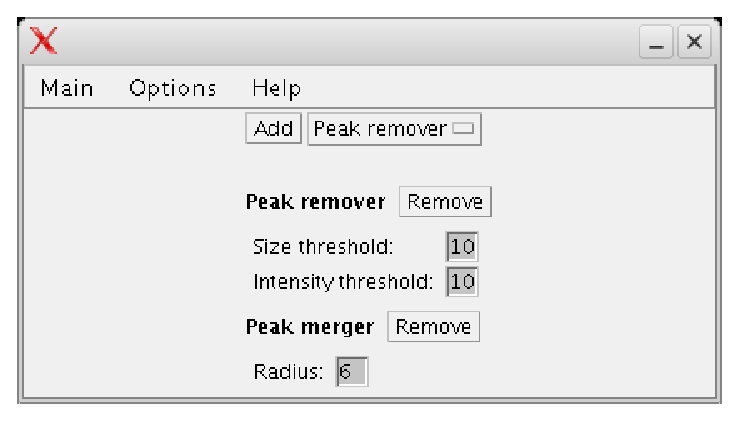
\includegraphics[width=0.5\columnwidth]{figures/GUI_post.eps}
\caption{Graphical user interface for Costanza.}
\label{fig:gui}
\end{center}
\end{figure}
%

\subsubsection{Input-Output}

This view allows for selecting input and output options. As input the active
stack is automatically chosen for segmentation. If an additional stack is to
be used for measuring intensities, the box ``use secondary stack...'' have to
be checked.

As default, the segmentation result is provided in a table displayed by
ImageJ. Additionally other types of output can be selected:

\begin{itemize}
%
\item Cell centers can be marked with red dots.
%
\item Basin of Attractions (BOAs), leading to the different cell centers can be
	displayed with random colors.
%
\item BOAs can be displayed with colors from measured intensities can be
	displayed. The color schema is from blue via green yellow to red.
%
\item The working stack can be displayed. This can be useful to see how the
	preprocessing has changed the original stack.
%
\end{itemize}

\subsubsection{Pre-processing}

Here different pre-processing step can be chosen, added and removed by the
user. The alternatives at the moment are:

\begin{itemize}
%
\item Invert, inverts the pixels in the stack. This is needed if the objects
	are dark in a brighter background, e.g. if bright membranes are marking
	cells.
%
\item Background threshold, this will set all pixels below a threshold
	intensity to belong to the background, and hence will not be available in
	the segmentation.
%
\item Mean Filter, this will reduce noise in the images by applying a mean
	filter with provided radius. As it is often useful to apply this more than
	once, this option is also provided by the user.
%
\end{itemize}

\subsubsection{Post-processing}

After the gradient descent algorithm is applied for segmentation, it might be
useful to do some post-processing. The available algorithms that can be
chosen, added and removed are:

\begin{itemize} 
%
\item Removal, where found compartments can be removed due to being too small
	or having too low intensity.
%
\item Merger, where compartments with centers too close to each other can be
	merged into a single compartment.
%
\end{itemize}

\section{Examples}

The performance of the Costanza application is dependent on the
parameters given to the different algorithms used. Here we provide
some examples of applications where also the parameter values used are
presented to guide users into setting reasonable parameter values.

\subsection{SAM nuclei data in 3D}

This data set represents nuclei marked cells in the Arabidopsis shoot apical
meristem. The data set consists of a stack with 20 images, but here the result
will be displayed in 2D images for an easier check on performance. The
segmentation is run using two different resolutions, and the result is shown
in Fig.~\ref{fig:43zoom}.

\begin{figure}[h!]
\begin{center}

\includegraphics[width=0.25\columnwidth]{figures/43smallzoomCenters.eps}
\hspace{0.20\columnwidth}
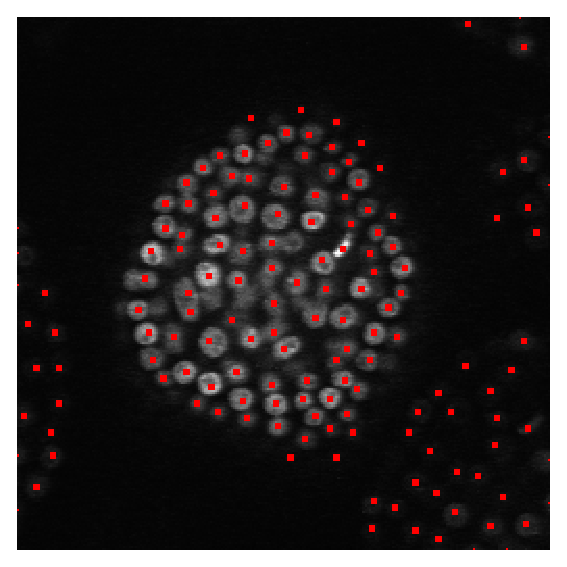
\includegraphics[width=0.5\columnwidth]{figures/43zoomCenters.eps}
\caption{Result shown for images of nuclei data. Original images can be found
	at http://www.thep.lu.se/...}
\label{fig:43zoom}
\end{center}
\end{figure}
%
Parameters used for these two runs are given in Table~\ref{tab:43zoom}, and
represents reasonable values also for 3D stacks.

\begin{table}
	\begin{center}
		\begin{tabular}{|l|cc|}
			\hline
			Parameter & Small & Large\\
			\hline
			Bg threshold & 10 & 10\\
			MeanFilter R & 1.0 & 2.5\\
			MeanFilter num & 2 & 2\\
			Remove Int Th. & 10 & 10\\
			Remove Size Th. & 5 & 10\\
			Merger R & 3 & 6\\
			xy-scale & 1 & 1\\
			z-scale & 1 & 2\\
			\hline
		\end{tabular}
		\caption{Nuclei extraction in 2D and 3D.}
		\label{tab:43zoom}
	\end{center}
\end{table}

\subsection{SAM membrane data in 2D}

This data set represents membrane marked cells in the Arabidopsis shoot apical
meristem. The data set consists of single images. The segmentation is run
using two different resolutions, and the result is shown in
Fig.~\ref{fig:membrane}.

\begin{figure}[h!]
\begin{center}
%\includegraphics[width=0.25\columnwidth]{figures/wus.eps}
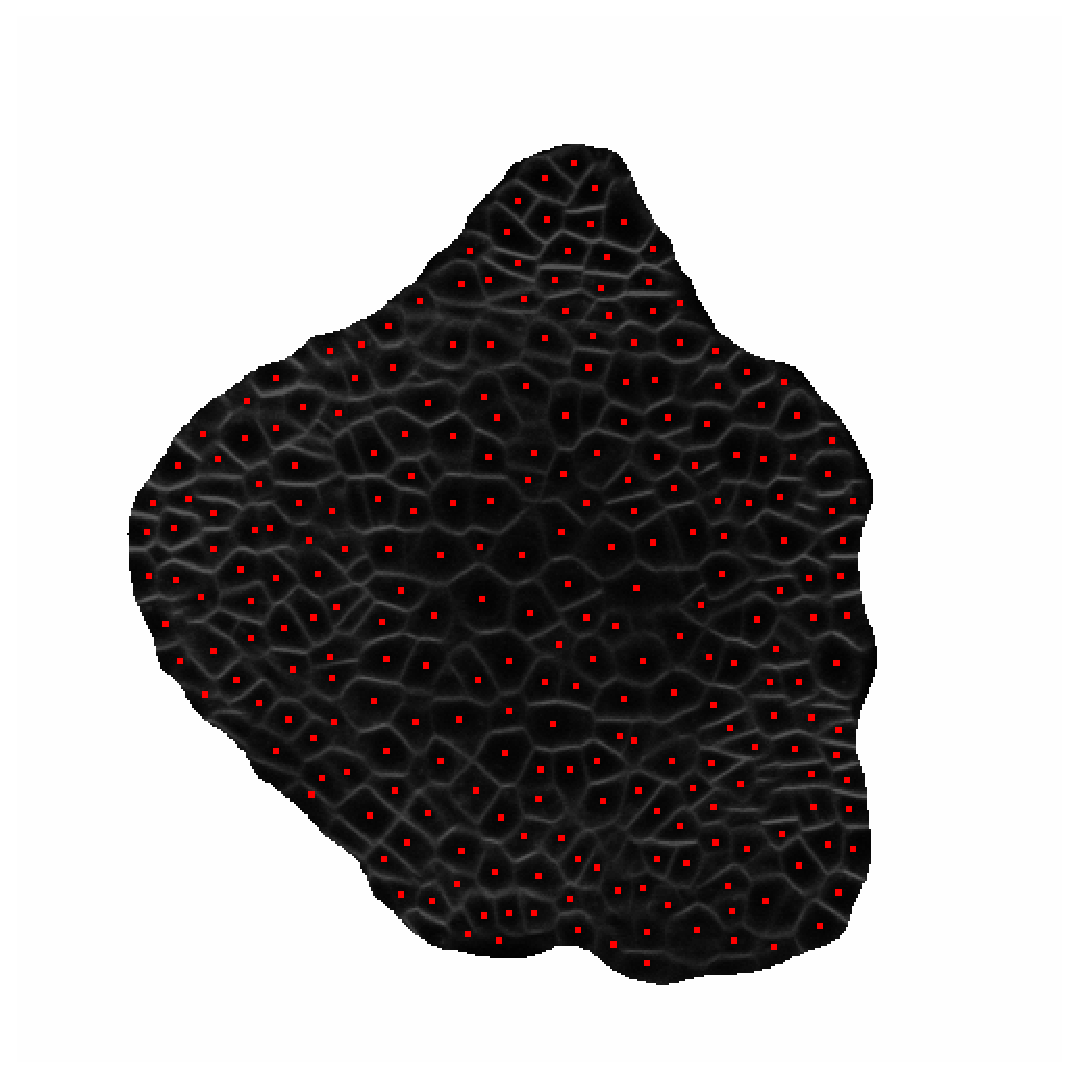
\includegraphics[width=0.25\columnwidth]{figures/wusCenters.eps}
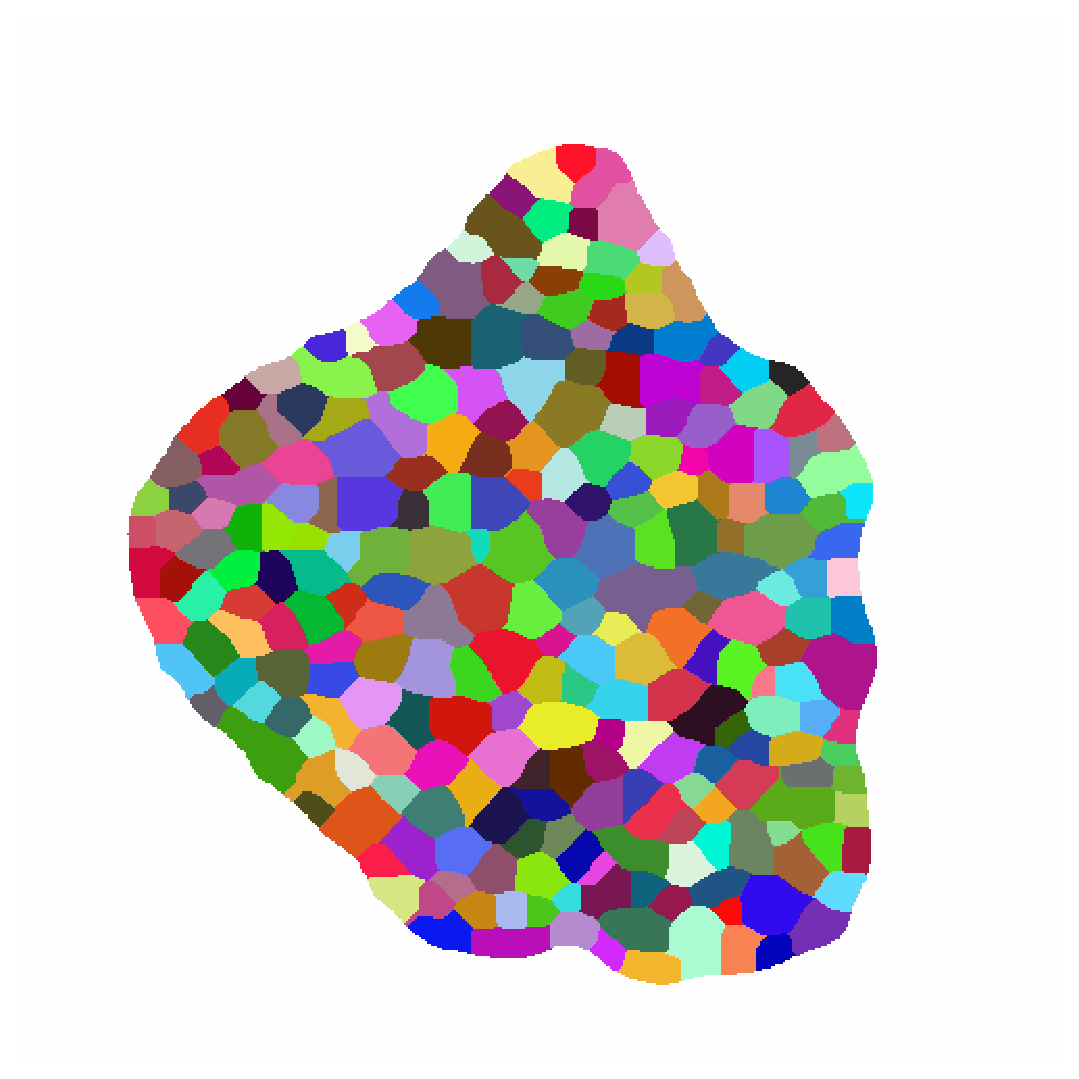
\includegraphics[width=0.25\columnwidth]{figures/wusBOAs.eps}
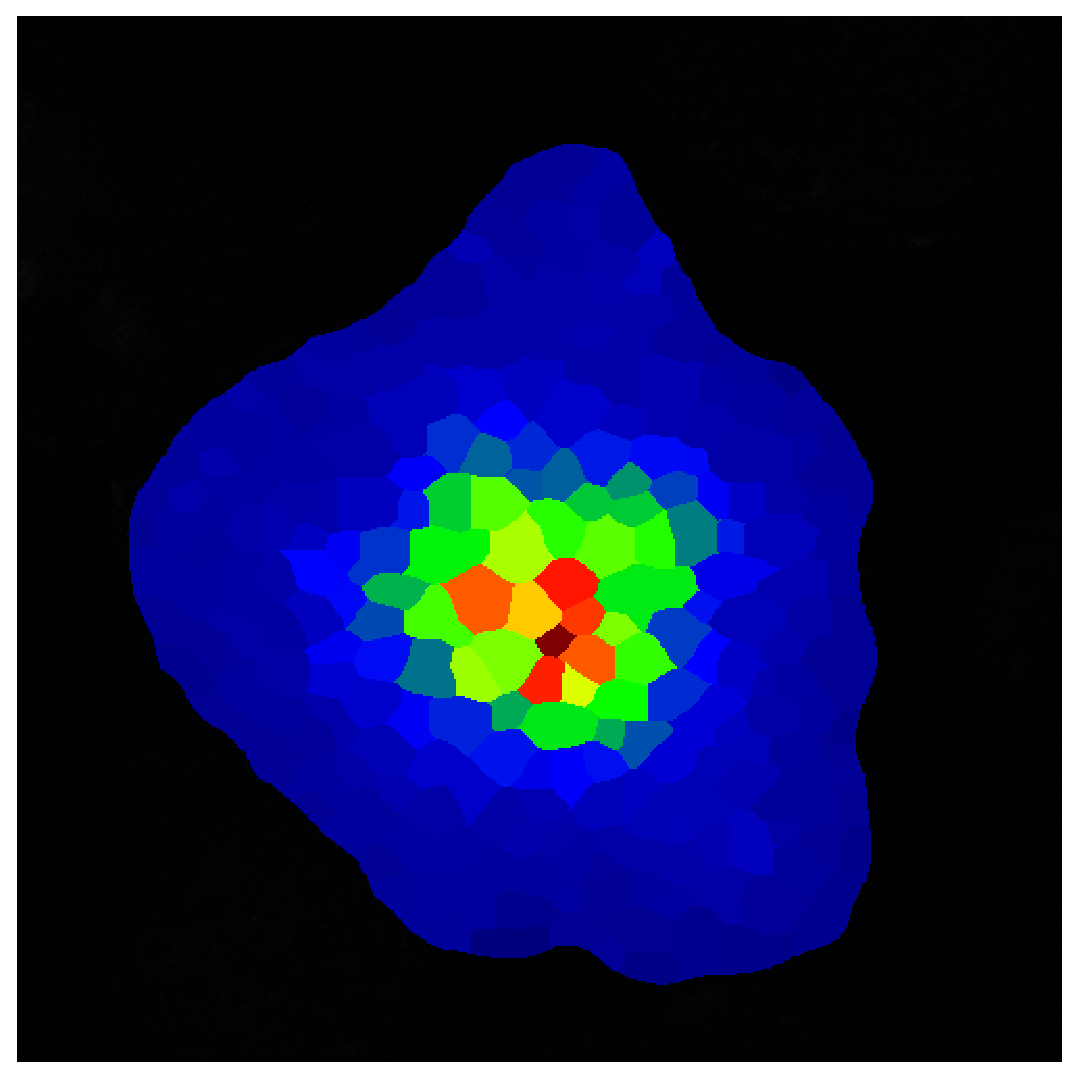
\includegraphics[width=0.25\columnwidth]{figures/wusBOAsIntensity.eps}

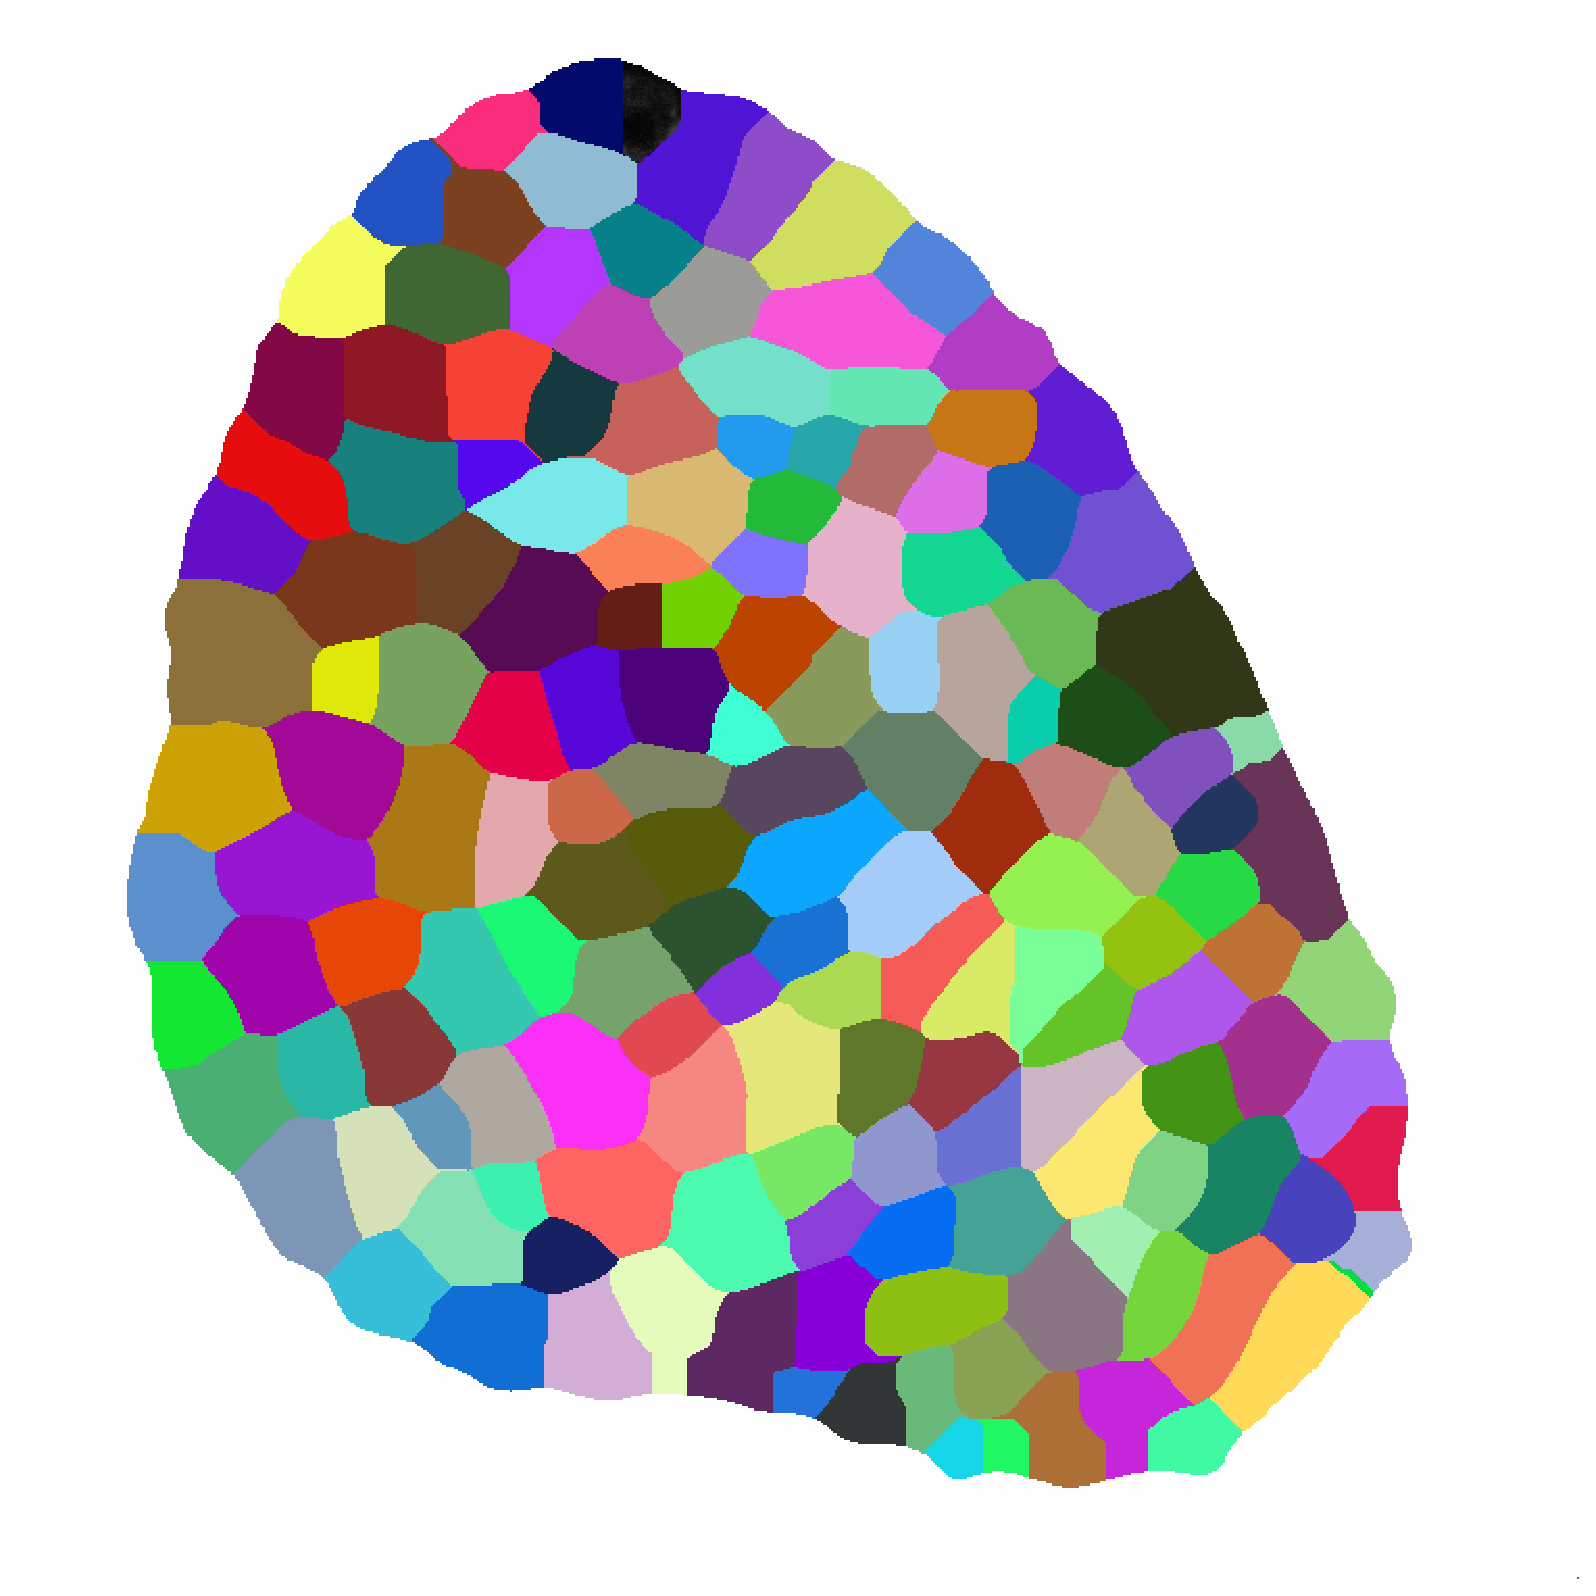
\includegraphics[width=0.33\columnwidth]{figures/pin1BOAs.eps}
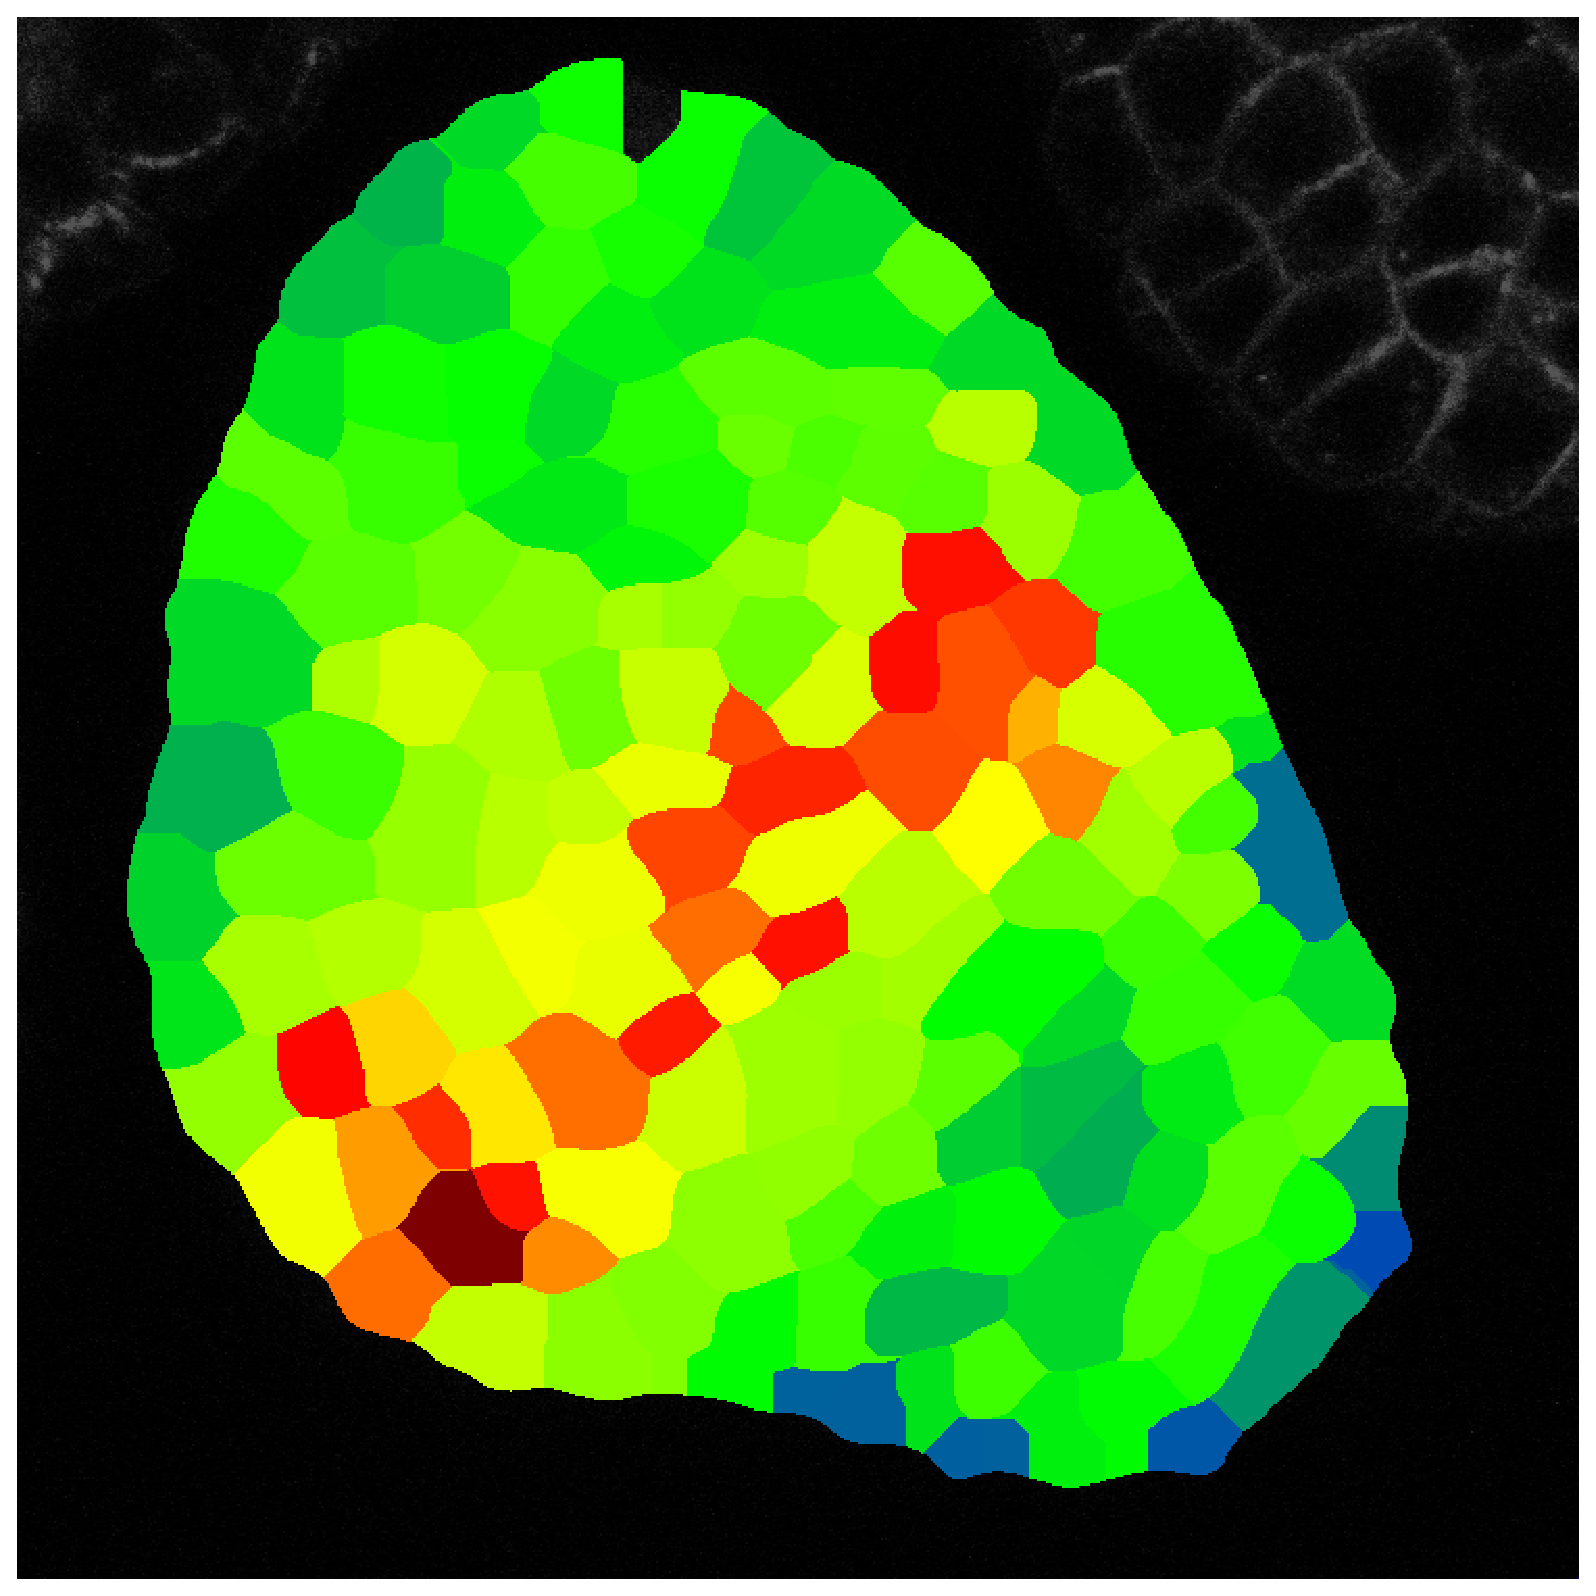
\includegraphics[width=0.33\columnwidth]{figures/pin1BOAsIntensity.eps}

\caption{Result shown for images of membrane data. Original images can be
	found at http://www.thep.lu.se/...}
\label{fig:membrane}
\end{center}
\end{figure}
%
Parameters used for these two segmentations are given in Table~\ref{tab:membrane}.

\begin{table}
	\begin{center}
		\begin{tabular}{|l|cc|}
			\hline
			Parameter & WUS & PIN1\\
			\hline
			Bg threshold & 1 & 1\\
			MeanFilter R & 5.0 & 10.0\\
			MeanFilter num & 2 & 2\\
			Remove Int Th. & 10 & 10\\
			Remove Size Th. & 10 & 10\\
			Merger R & 5 & 10\\
			xy-scale & 1 & 1\\
			z-scale & - & -\\
			\hline
		\end{tabular}
		\caption{Cell extraction in 2D membrane data.}
		\label{tab:membrane}
	\end{center}
\end{table}

\bibliographystyle{abbrv}
\bibliography{references}

\end{document}
